\subsection{The clench, on real recordings}
\label{sec:clench}

\begin{figure}[t]
\centering
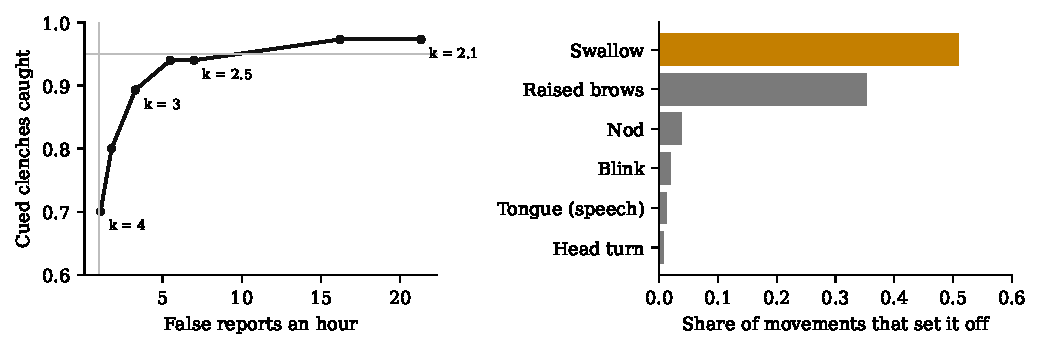
\includegraphics[width=\linewidth]{fig_clench.pdf}
\caption{The phone's clench detector, unchanged. Left: around the ear (15 people, 250~Hz), cued 3~s clenches caught against false reports an hour in blinking, eye movements, rest and heartbeat, for thresholds $k$ from 2.1 to 4 (shipped); grey lines mark the bars of 95\% caught and one false report an hour. Right: the share of each labelled movement during which it reported a gesture (12 people, temporal scalp, 1000~Hz).}
\label{fig:clench}
\end{figure}

At the shipped threshold the detector caught \clAround{} of cued clenches around the ear, \clHeadband{} on a consumer headband with one electrode behind each ear, and \clScalp{} of cued clench blocks on the temporal scalp at 1000~Hz. Around the ear the misses were concentrated: ten of fifteen people had nine or ten of their ten clenches caught, five had three or fewer, and in those five the muscle signal of the weaker ear rose only 2.4 to 3.9 times above its background during a clench, under the threshold of four. Lowering the threshold catches them and costs false reports (Figure~\ref{fig:clench}, left): \clAroundThree{} of clenches at \clAroundThreeFalse{} false an hour for $k=3$, against \clAroundFourFalse{} for $k=4$. A personal threshold set from each person's first three clenches did not reliably beat a fixed one: chosen on half the people it caught every later clench at 1.4 false an hour, and on the other half 84\% at 7.1.

Every recording without a cued clench measures false reports. In 89 minutes of rest and heartbeat around the ear there were three, in 74 minutes of blinking and eye movement none, and on the headband none at rest, six an hour while blinking and fifteen while moving the head. In \clListenHours{} hours of quiet listening (ds004015, 500~Hz, the earbud's four electrodes per ear) there were \clListen{} an hour: the median listener two, the worst 37. By labelled movement, swallowing set the detector off \clSwallow{} of the time and raised eyebrows \clBrows{}, while tongue movement as in speech did \clTongue{}, head nods and turns 0.7 to 3.8\%, blinks 1.9\% and eye movements never (Figure~\ref{fig:clench}, right).

Double clenches were the exception everywhere: \clListenDouble{} false doubles an hour in quiet listening against \clListenOthers{} singles and holds, none in the labelled movements apart from 2 of 452 tongue movements, and in every recording 20 to 50 times rarer than a false single.

Swallows could not be rejected in software. Described by what the detector could compute as it goes (the weaker ear's peak over its background, the time above half the peak, slow potentials during the event, upper against lower contacts, spectral balance and symmetry), the \clSwallowN{} labelled swallows and the \clClenchBursts{} bursts inside the cued clench blocks overlapped on every feature (the best single AUC \clSwallowBest{}), and all six together, trained on eleven people and tested on the twelfth, reached an AUC of \clSwallowAuc{}: keeping 95\% of clenches would have rejected \clSwallowKeep{} of swallows.
